\begin{figure}\begin{center}
		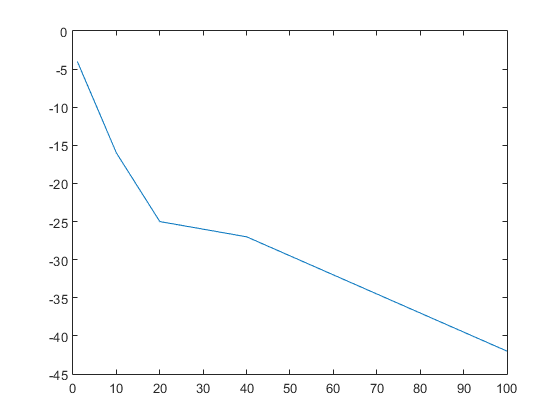
\includegraphics[width=\figurewidth]{plots/can_p.png}
		\caption{Our cantenna. Measured signal strength depending on the distance. Horizontal axis in meters, vertical axis in dBm.}
		\label{img:dist:pow:can}
		
		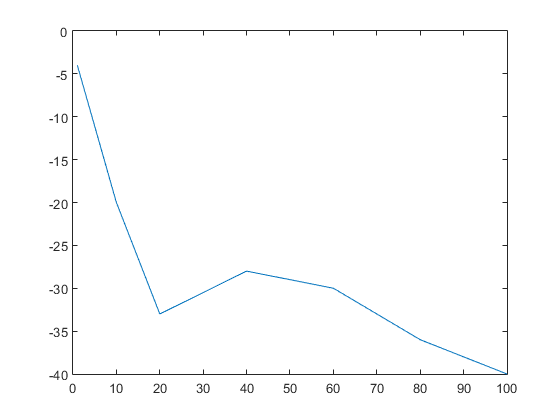
\includegraphics[width=\figurewidth]{plots/prof_p.png}
		\caption{Professional cantenna. Measured signal strength depending on the distance. Horizontal axis in meters, vertical axis in dBm.}
		\label{img:dist:pow:prof}
		
		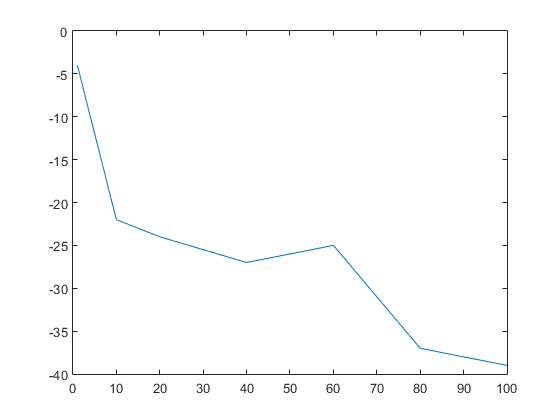
\includegraphics[width=\figurewidth]{plots/omni_p.png}
		\caption{Omni-directional cantenna. Measured signal strength depending on the distance. Horizontal axis in meters, vertical axis in dBm.}
		\label{img:dist:pow:omni}
	\end{center}\end{figure}
	
	%distance bandwidth
	\begin{figure}\begin{center}
			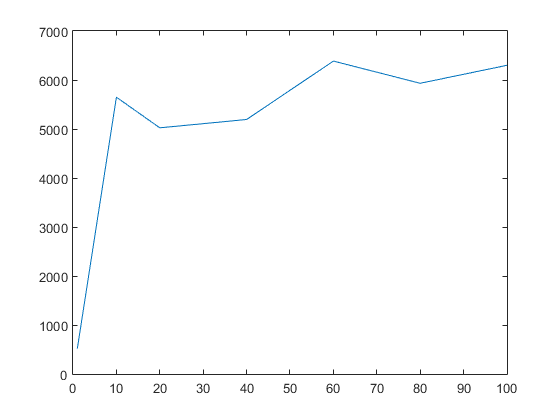
\includegraphics[width=\figurewidth]{plots/can_b.png}
			\caption{Our cantenna. Measured bandwidth depending on the distance. Horizontal axis in meters, vertical axis in Kib/s.}
			\label{img:dist:band:can}
			
			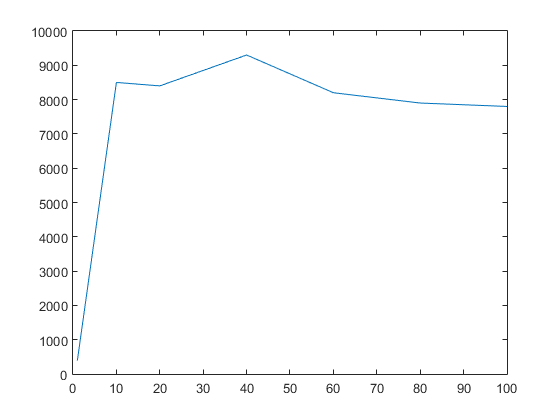
\includegraphics[width=\figurewidth]{plots/prof_b.png}
			\caption{Professional cantenna. Measured bandwidth depending on the distance. Horizontal axis in meters, vertical axis in Kib/s.}
			\label{img:dist:band:prof}
			
			
			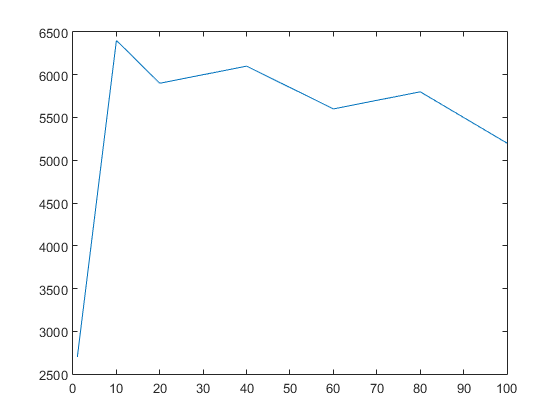
\includegraphics[width=\figurewidth]{plots/omni_b.png}
			\caption{Omni-directional cantenna. Measured 1bandwidth depending on the distance. Horizontal axis in meters, vertical axis in Kib/s.}
			\label{img:dist:band:omni}
		\end{center}\end{figure}
		
		%angular pow
		\begin{figure}\begin{center}
				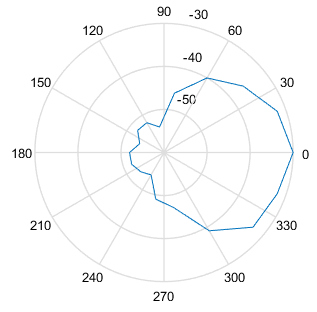
\includegraphics[width=.45\textwidth]{plots/cantenna_power_cut.png}
				\caption{Our cantenna. Measured signal strength depending on the angle. Polar axis in degree, radius axis in dBm.}
				\label{img:ang:pow:can}
				
				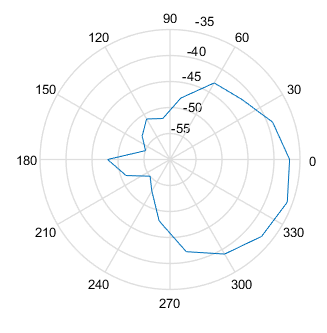
\includegraphics[width=.45\textwidth]{plots/prof_power_cut.png}
				\caption{Professional cantenna. Measured signal strength depending on the angle. Polar axis in degree, radius axis in dBm.}
				\label{img:ang:pow:prof}
				
				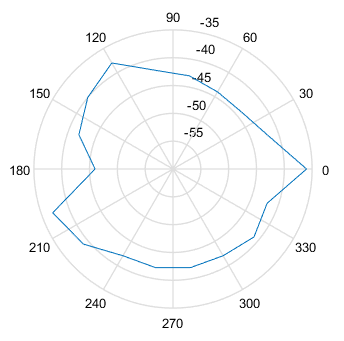
\includegraphics[width=.45\textwidth]{plots/poer_omni_cut.png}
				\caption{Omni-directional cantenna. Measured signal strength depending on the angle. Polar axis in degree, radius axis in dBm.}
				\label{img:ang:pow:omni}
			\end{center}\end{figure}
			
			%angular bandwidth
			\begin{figure}\begin{center}
					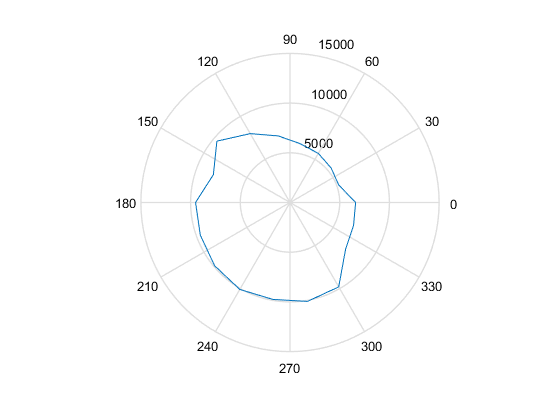
\includegraphics[width=\figurewidth]{plots/polar_can_b.png}
					\caption{Our cantenna. Measured bandwidth depending on the angle. Polar axis in degree, radius axis in Kib/s.}
					\label{img:ang:band:can}
					
					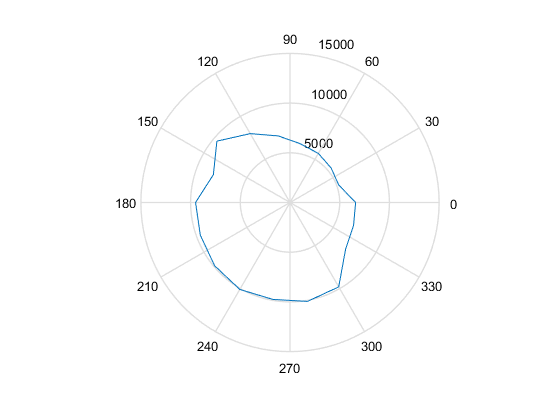
\includegraphics[width=\figurewidth]{plots/polar_prof_b.png}
					\caption{Professional cantenna. Measured bandwidth depending on the angle. Polar axis in degree, radius axis in Kib/s.}
					\label{img:ang:band:prof}
					
					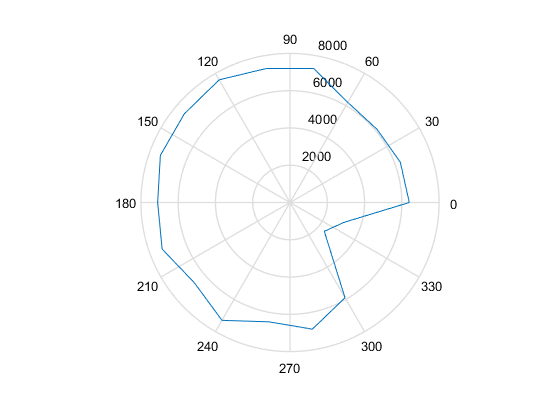
\includegraphics[width=\figurewidth]{plots/polar_omni_b.png}
					\caption{Omni-directional cantenna. Measured bandwidth depending on the angle. Polar axis in degree, radius axis in Kib/s.}
					\label{img:ang:band:omni}
				\end{center}\end{figure}